\documentclass{standalone}
\standaloneconfig{border=2mm 2mm 2mm 2mm}


%maths
\usepackage{mathtools}
\usepackage{amsmath}
\usepackage{amssymb}
\usepackage{amsfonts}

%tikzpicture
\usepackage{tikz}
\usepackage{scalerel}
\usepackage{pict2e}
\usepackage{tkz-euclide}
\usetikzlibrary{calc}
\usetikzlibrary{patterns,arrows.meta}
\usetikzlibrary{shadows}
\usetikzlibrary{external}

%pgfplots
\usepackage{pgfplots}
\pgfplotsset{compat=newest}
\usepgfplotslibrary{statistics}
\usepgfplotslibrary{fillbetween}

%colours
\usepackage{xcolor}

\usepackage{nicefrac}

\begin{document}
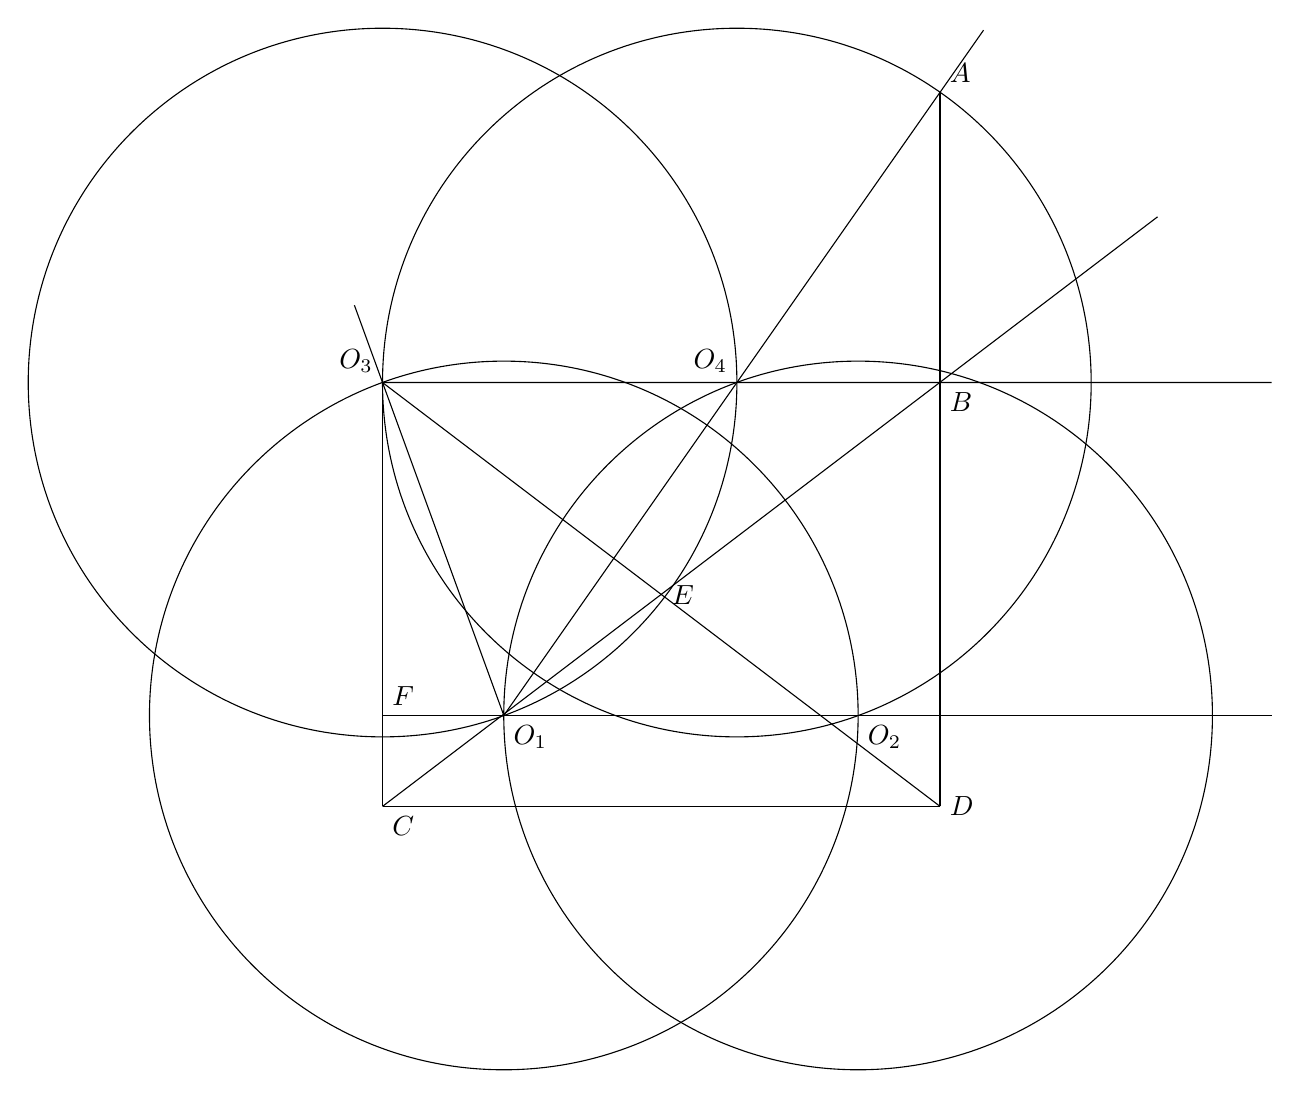
\begin{tikzpicture}[scale=1.5]

\coordinate [label=below right:{$O_1$}] (O_1) at (0, 0);
\coordinate [label=below right:{$O_2$}] (O_2) at (3, 0);
\coordinate [label=above left:{$O_3$}] (O_3) at (-1.026694933997, 2.8188468409094);
\coordinate [label=above left:{$O_4$}] (O_4) at (1.973305066003, 2.8188458409094);
\coordinate [label=above right:{$F$}] (F) at (-1.026694933997, 0);
\coordinate [label=below right:{$C$}] (C) at (-1.026694933997, -0.7698231815855);
\coordinate [label=right:{$D$}] (D) at (3.6937577968284, -0.7698231815855);
\coordinate [label=above right:{$A$}] (A) at (3.6937577968284, 5.2764966127434);
\coordinate [label=below right:{$B$}] (B) at (3.6937577968284, 2.8188468409094);
\coordinate [label=right:{$E$}] (E) at (1.3396305141736, 1.0217647555776);

\draw (O_1) circle [radius=3];
\draw (O_2) circle [radius=3];
\draw (O_3) circle [radius=3];
\draw (O_4) circle [radius=3];

\draw (O_3)--(C);
\draw (O_3)--(6.5, 2.8188468409094);
\draw (F)--(6.5, 0);
\draw (C)--(D);
\draw (O_1)--(4.06156427, 5.8019045);
\draw (D)--(A);
\draw (D)--(O_3);
\draw (O_1)--(-1.2651009, 3.4734034);
\draw (C)--(5.534707, 4.221439);

\end{tikzpicture}
\end{document}
